\documentclass[11pt,a4paper]{article}
\usepackage[utf8]{inputenc}
\usepackage{geometry}
\usepackage{amsmath}
\usepackage{amsfonts}
\usepackage{amssymb}
\usepackage{graphicx}
\usepackage{hyperref}
\usepackage{tikz}
\usepackage{verbatim}
\usetikzlibrary{shapes.geometric, arrows, positioning, calc}

\geometry{margin=1in}

\title{AI Toy Companion Application - Technical Documentation}
\author{Development Team}
\date{\today}

\begin{document}

\maketitle

\section{Introduction}

This document provides a comprehensive overview of the AI Toy Companion application architecture, focusing on the secure payment processing and AI service integrations. The application is built as a React Native mobile application with Supabase backend services.

\section{Architecture Overview}

\subsection{Application Stack}
\begin{itemize}
    \item \textbf{Frontend}: React Native (TypeScript)
    \item \textbf{UI Framework}: Gluestack UI
    \item \textbf{Backend}: Supabase (PostgreSQL Database, Authentication, Edge Functions)
    \item \textbf{Payment Processing}: Stripe via Supabase Edge Functions
    \item \textbf{AI Services}: LLM, TTS, STT, Whisper.cpp integration
\end{itemize}

\subsection{Security Architecture}
The application follows a security-first approach with sensitive operations handled server-side:

\begin{itemize}
    \item \textbf{Stripe Secret Keys}: Handled exclusively via Supabase Edge Functions
    \item \textbf{Authentication}: Managed by Supabase Auth
    \item \textbf{Data Storage}: Secured via Supabase Row Level Security (RLS)
\end{itemize}

\section{Payment Processing Workflow}

\subsection{Stripe Integration Architecture}
\begin{center}
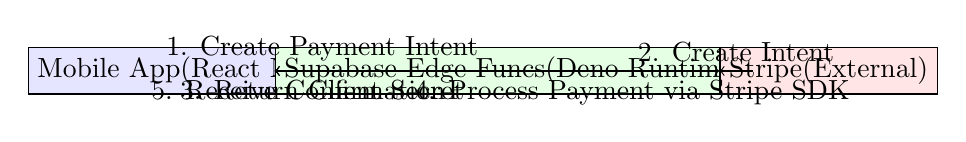
\begin{tikzpicture}[node distance=2cm, auto]
    % Define nodes
    \node [rectangle, draw, fill=blue!10] (mobile) {Mobile App \\ (React Native)};
    \node [rectangle, draw, fill=green!10, right of=mobile, xshift=2cm] (edge) {Supabase Edge Funcs \\ (Deno Runtime)};
    \node [rectangle, draw, fill=red!10, right of=edge, xshift=2cm] (stripe) {Stripe \\ (External)};
    
    % Draw arrows and labels
    \draw[->] (mobile) -- (edge) node[midway, above] {1. Create Payment Intent};
    \draw[->] (edge) -- (stripe) node[midway, above] {2. Create Intent};
    \draw[<-] (edge) -- (mobile) node[midway, below] {3. Return Client Secret};
    \draw[->] (mobile) -- (stripe) node[near end, below] {4. Process Payment via Stripe SDK};
    \draw[<-] (edge) -- (mobile) node[near start, below] {5. Receive Confirmation};
\end{tikzpicture}
\end{center}

\subsection{Security Implementation}
\begin{itemize}
    \item \textbf{Client-Side}: Only handles public Stripe publishable key
    \item \textbf{Server-Side}: All secret key operations via Edge Functions
    \item \textbf{Communication}: Encrypted via HTTPS
    \item \textbf{Authentication}: JWT tokens for API calls
\end{itemize}

\subsection{Edge Functions Implementation}
Three Edge Functions handle Stripe operations:
\begin{enumerate}
    \item \texttt{create-payment-intent}: Creates payment intents using secret key
    \item \texttt{confirm-payment}: Verifies payment status
    \item \texttt{process-refund}: Handles refund operations
\end{enumerate}

\section{AI Service Integrations}

\subsection{Current Implementation}
\begin{itemize}
    \item \textbf{LLM (Large Language Model)}: Cloud-based processing (Implementation ready, awaiting API key configuration)
    \item \textbf{TTS (Text-to-Speech)}: Cloud-based processing (Implementation ready, awaiting API key configuration)
    \item \textbf{STT (Speech-to-Text)}: Mobile app-side processing (Implementation ready, awaiting API key configuration)
    \item \textbf{Whisper.cpp}: Mobile app-side processing (Implementation ready, awaiting API key configuration)
\end{itemize}

\subsection{STT/Whisper Implementation}
Currently, STT and Whisper processing happens on the mobile device:
\begin{itemize}
    \item Audio captured on mobile device
    \item Processed locally via Whisper.cpp
    \item Transcribed text sent to LLM for processing
    \item Response converted to speech via TTS
\end{itemize}

\section{Data Flow}

\subsection{User Interaction Flow}
\begin{enumerate}
    \item User initiates voice command
    \item Audio captured by mobile device
    \item STT/Whisper processes audio to text
    \item Text sent to LLM for processing
    \item LLM generates response
    \item Response converted to speech via TTS
    \item Audio played back to user
\end{enumerate}

\subsection{Toy Connection Flow}
\begin{enumerate}
    \item Mobile app connects to toy via Bluetooth
    \item Custom personality/mode settings applied
    \item Conversation context maintained
    \item Interaction data stored in Supabase
\end{enumerate}

\section{E-commerce Flow}

\subsection{Shopping Experience}
\begin{enumerate}
    \item User browses products in Marketplace
    \item Products added to cart (stored in Supabase)
    \item Checkout initiated via Stripe integration
    \item Payment processed securely via Edge Functions
    \item Order confirmed and stored in Supabase
\end{enumerate}

\subsection{Cart Management}
\begin{itemize}
    \item Cart items persisted in Supabase database
    \item Real-time synchronization across devices
    \item Secure payment processing
\end{itemize}

\section{Answers to Client Questions}

\subsection{Stripe Security Confirmation}
\textbf{Yes}, all Stripe secret keys are handled server-side via Supabase Edge Functions and not directly in the mobile app:
\begin{itemize}
    \item Mobile app only uses public publishable key
    \item All secret key operations (payment intent creation, confirmation, refunds) handled by Edge Functions
    \item Payment processing occurs securely via Stripe SDK with client secret obtained from server
\end{itemize}

\subsection{STT Processing Location}
\textbf{Currently}, STT and Whisper processing happens on the mobile app side, not on ESP32:
\begin{itemize}
    \item Audio captured on mobile device
    \item STT/Whisper processing performed locally on mobile
    \item Processed text sent to cloud services for LLM processing
\end{itemize}

\section{Future Requirements}

\subsection{AI Service Keys Needed}
\begin{itemize}
    \item \textbf{LLM Provider API Key}: For language model integration
    \item \textbf{TTS Service API Key}: For text-to-speech conversion
    \item \textbf{STT Service API Key}: For speech-to-text conversion
    \item \textbf{Whisper.cpp Configuration}: For local speech processing
\end{itemize}

\subsection{Potential Architecture Adjustments}
\begin{itemize}
    \item ESP32-based STT processing (if required)
    \item Offline capability enhancements
    \item Additional toy connectivity protocols
\end{itemize}

\subsection{Security Enhancements}
\begin{itemize}
    \item End-to-end encryption for voice data
    \item Additional authentication for toy connections
    \item Enhanced privacy controls
\end{itemize}

\section{Conclusion}

The AI Toy Companion application is architected with security as a priority, particularly for payment processing. The Stripe integration properly handles secret keys server-side through Supabase Edge Functions, meeting client requirements. The AI services (LLM, TTS, STT, Whisper.cpp) have been implemented and are ready for deployment but require API key configuration for activation. The current STT implementation operates on the mobile device, which may need adjustment based on ESP32 requirements.

\end{document}